\documentclass[12pt]{article}
\usepackage[margin=1in]{geometry}
\usepackage{graphicx}
\graphicspath{ {./} }


\title{Talkatiel Software Requirements and Planning}
\author{Brendan Byers, Ryan Sisco, Iliana J, Aidan Grimshaw}
\date{\today}

\begin{document}
\begin{center}
 \Large\textbf{Talkatiel Second Implentation System}\\
 \large\textit{Brendan Byers, Ryan Sisco, Iliana J, Aidan Grimshaw, Yufei Zeng}\\
 \large{byersbr, siscor, javieri, grimshaa, zengyu}\\
\end{center}

\tableofcontents
\section{Product Release} \subsection{Server Side Implementation} Currently the
server code can be downloaded and run locally.  By cloning the repository
located at\begin{verbatim} https://github.com/B13rg/Talkatiel_API.git
\end{verbatim}one can run the server.  There is also extensive documentation
detailing all the steps that need to be taken to run the server.  There is also
a SQL script that will create a database when run.  This can be used to create a
database for use on a different engine.  Currently it is configured to run on
the localhost on port 5002.  This can be tested to navigating to
\begin{verbatim}127.0.0.1:5002/Posts/New \end{verbatim}where you can see the raw
Json output of a post.  In the repository there is also an sqlite database that
is run alongside the python code.  This will connect with the python to respond
to different sql queries.  It is fully functioning, and the only thing left to
do is test it, and find a permanent URL. Additionally, you can test GET and POST
reqeusts at our API server URL, aidangrimshaw.pythonanywhere.com, using the
documentation located on our API github repo.

\subsection{Client-Side Implementation}
By midweek, we plan to start permanent hosting with google app engine. Product
URL:\begin{verbatim} https://github.com/thegrims/talkatiel-ui \end{verbatim} The
product is current working on a basic level. We are able to consistently pull
data and connect to the server. We have added several test posts and are able to
bring them into cards on our mobile client. We are currently working on
developing our fingerprinting and identifying users individually and tying them
to their posts server side only. This will take some time and testing, and will
only be implemented after a series of testing and penetration testing. When we
implement this, we need to be absolutely sure that the data is secure, because
we will be dealing with sensitive data.

Our CSS is looking as intended. We have built it to be easy to change later on.
We are not completely decided on a color, however it works with most. We have
yet to implement animations. We do have screen rotation completed for mobile
devices, and the app grows in size accordingly. We have tested the app on IOS
and Android, with a consistent look between the two.

\section{User Story}

\subsection{Add a post}

A user can now add a post using the client side program.  They are able to set a 
title and text, and post it for everyone to see.  When it is sent to the server 
the server will add it to the database, so then it may be retrieved by other users.

As part of adding a post we wanted to filter out bad words.  This will help cut 
down on bullying in the online community of our project.  To do this we created 
a special function that takes a post's text and checks it against a wordlist.  
The wordlist is a seperate file so we are able to update as need be.  If we find 
new words we can just add them to the end of the list.  This means the client 
won't have to recompile the app every time we make a change to the wordlist.
\begin{center}
	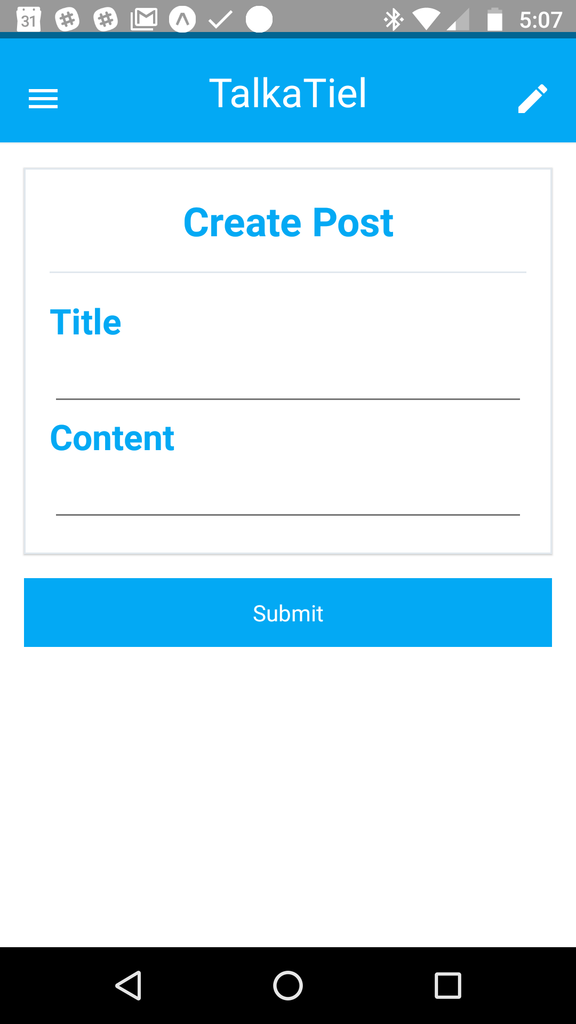
\includegraphics[scale=0.75]{img/create_post}\linebreak
	\textbf{Class Diagram}
\end{center}

\subsection{Add a Comment}

Adding a comment works the same way as adding a post.  A user will choose content 
for the comment and then it will be checked and sent to the server.  When comments 
are retrieved from the server, the server will return all child comments for a post.  
Before it would only return top level comments, but now they will be correctly 
tiered.  The comments will be displayed on the screen when people refresh the 
comments of a specific post.  In order to test this there are unit tests to test 
the server side of things.

\subsection{Like/Dislike}

\subsection{Report}

\subsection{Delete}

\subsection{Refresh}
Both the feed and refresh user stories are complete.  A user is now able to refresh the 
feed and view new posts.  In the image below, all the posts are test posts, but they are 
distinct.  The fact that this works means that both the client and server implimentations 
of creating a post and fetching posts are working.  Depending on the sort choice, posts 
will be sorted by Hot, New, and Top.  New simply returns the newest posts from the database 
but hot and top are calculated every 2 minutes.  This lowers the amount of queries the 
database needs to handle and instead allows the server to rely on the cache instead, which 
speeds up requests.  In order to test this there are unit tests to test the server side of things.
\begin{center}
	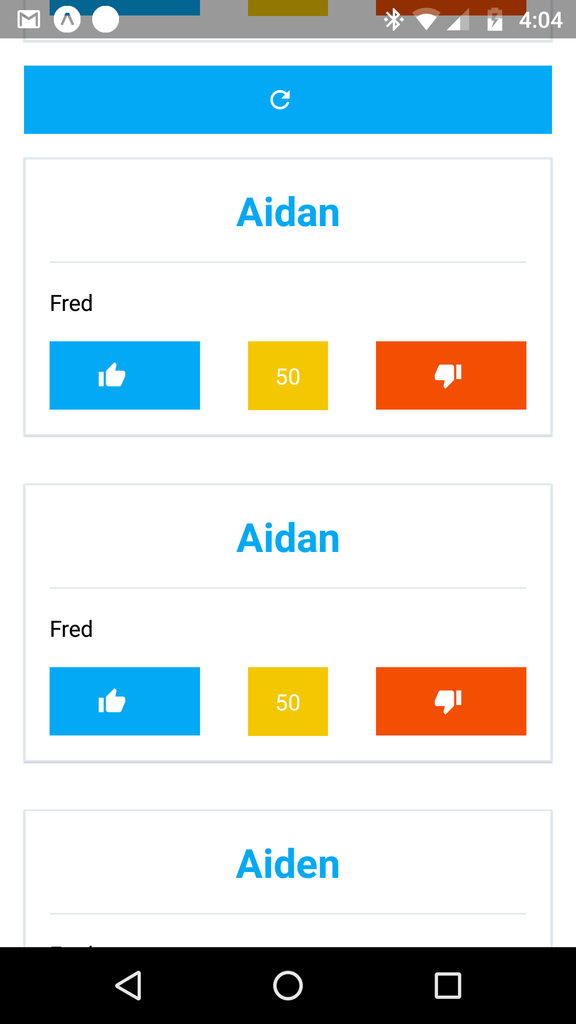
\includegraphics[scale=0.75]{img/view_posts}\linebreak
	\textbf{Class Diagram}
\end{center}

\subsection{Sort}

\subsection{View Newly Created Post}
Because of how sorting by new is implemented, a user is able to see their posts immediately.  
This is because there is no caching done on that sorting method.  This makes it so the 
database is queried every time.  If the server load was a lot, it would still be acceptable 
to cache things for even 5 minutes to lighten the load on the server.  The client is now 
able to request posts, so the client is able to see their newly submitted post when requested.

\subsection{Secure HTTPS Connection}

Luckily, this user story wasn't too difficult in the end.  The url where the server is hosted 
allows for https connections without any setup from us.  Therefore, we are able to blacklist 
all requests that are not through SSL.  This means that in order to make a request to the 
server, it needs to be made using https.  This will make sure that all content to and from the 
server is delivered over a secure connection.  It is nice that the Python Anywhere service has 
this ability, else we would need to genereate and sign the certificates ourselves which can be 
time consuming if done incorrectly.

\subsection{Save Website as App on Phone}

\subsection{Responsive Web Page}

\section{Tests}

The server side of this project calculates and delivers it to the client.
Therefore, it is important to properly test the API service so that it either
returns the complete set of data or returns an error.  It is relativly easy to
test this.  A script was created that goes through and tests each part of the
API.  First it checks to see if the API is online.  It does this by using the
Ping tool to test the url of the API, in this case
\begin{verbatim}http://aidangrimshaw.pythonanywhere.com \end{verbatim}.  This
determines if the aPI is even able to recieve anything.  Next it goes through
each part of the API and checks to make sure it works.  This portion is done
using the CURL tool.  The command used looks something like:

\begin{verbatim} curl -H \"Content-Type: application/json\" -X POST -d \'{
\"content\": \"Fred\",\"userID\": 343434,\"title\":\"Aiden\"}'
http://aidangrimshaw.pythonanywhere.com/Posts \end{verbatim}

This will make a POST request with data to the server.  This data will be added
to the database.  The \"-H \'Content-Type: application/json\" declares that the
header for the request markes the content type as json.  This will signal to the
server to look for a data section and parse it as Json.  The \"-X POST\" marks
what type this request is.  Because there is a data section curl assumes it is a
POST request, but it is good to mark this just in case.  The \"-d\" marks the
beginning of the data section, and you can see the raw json data that is passed
to the server.  Finally, there is the URL address to send this request to.  For
each POST and GET outlet in the API there is a specific curl test for it.  The
script runs each of the tests and records the response.  The server responds
with how the request went, and will signal to the client if it was successful.
If is not successful, the server will alert the client that the request failed.
We are able to parse whatever response the server makes and record it with the
test.  After all the tests are run, the script looks at which tests failed,
lists them, and prints any extra data it recieved.  This could be response data
or error codes.  This allows us to quickly test the server when we make changes
to confirm that nothing was broken.

\section{Design Changes and Rationale}
\subsection{Server Side Implementation}
For the most part the server group stayed very close to original design.  To
design the database, we worked off the UML design diagrams we designed earlier.
This allowed us to see what fields we needed to include for each table.  We
added an extra table not originally in the design doc to handle reports.  We
found there was no way to keep track of reports server side, so we added a table
to handle it.  It keeps track of the user who reported it, the post in question,
and the text of the user’s report.  By having its own table, it can also be
queried separately instead of having to sort through who knows what.
Additionally, we modified our api server implementation so that it was served
remotely from a different service than the client side server, and so that the
API would be better equiped to handle POST requests.
\subsection{Frontend Implementation}
We have stayed very close to our original design. We currently are finishing up
our implementation of the main posts page, and will switch our focus to the
implemetation of the posts page and further code cleanup / refactoring of the
posts page. Visual elements are styled slightly differently for ease of use, and
commenting functionality is removed in this version to ease the implementation
of our minimum viable product (MVP).

\section{Refactoring}

Our project is still being developed in parts. For the most part, we have
been working towards building a working application and database, and slowly
cleaning up as we go. This has lead to some sloppy, duplicate code. However,
we have been making progress building. Once one of our members has completed
his/her section, while waiting for others to complete, they have cleaned up
their code and make it easier to follow. While this isn’t a top priority
right now, we believe that refactoring our code as we complete files will
help us in the future. It will also allow us to switch duties and work on
each other's code without too much confusion.

We ended up doing minor refactoring. While working on the client side
development, we ended up making templates for common, reoccurring elements.
This has been useful while developing other parts of the application, when
attempting to make the styling similar. We have been able to remain somewhat
consistent.

In addition to these changes, we have also changed variable names before
committing to the shared repository. This helps those who are viewing
changes follow along. Many of us have been saving files offline before
pushing, forcing us to correct changes before pushing. By doing this, we are
not stressed to push our work as a simple “backup” of our work. Saving and
updating locally/remotely before pushing to a shared repo has helped us stay
consistent and organized.

Making these changes has helped us stay organized and also limit the
“turnover” time between switching parts and tasks. For instance, when two
people switched files to review code, we were able to follow along much
easier when the code was simplified.

\section{Meeting Report}
\subsection{Progress Made this Week}

This week we continued to work on implementing our project as well as beginning 
to test the software. We have completed most user stories created for this 
project. The front end team created the basic UI and implemented scrolling and 
button pressing interactions. More features such as screen rotation and making 
sure the UI works on both IOS and Android were also implemented. Back end team 
set up a temporary server running on two laptops and ported the application to 
mobile.  

Project release and Refactoring statements were also written.  


\subsection{Plans for Next Week}

Next week we will wrap up the implementation of our app.  We will work on making
sure all the aspects of the project work well together.  This means more integration
tests and making sure there are as few bugs as possible.

\subsection{Team Member Contributions}

Server - Brendan Byers, Aiden Grimshaw, Ryan Sisco

UI  - Aiden Grimshaw

Testing - Brendan Byers

Product Release - Ryan Sisco

Meeting Report - Iliana Javier

User Stories - Yufei Zeng

\end{document}
